\documentclass[conference,letterpaper]{IEEEtran}

\usepackage{graphicx}
\usepackage{booktabs}
\usepackage{amsmath}
\usepackage{cite}
\usepackage[hidelinks]{hyperref}

\graphicspath{{figures/}}


\begin{document}

\title{Comparing a Support Vector Machine and a Multilayer Perceptron on the Dry Bean Dataset}

\author{\IEEEauthorblockN{Oluwasegun Adewola}
\IEEEauthorblockA{CS 5330: Pattern Recognition and Computer Vision\\
Northeastern University, Vancouver\\
adewola.ol@northeastern.edu}}

\maketitle

\begin{abstract}
I compare traditional classifiers and a multilayer perceptron (MLP) on the Dry Bean dataset, where each grain is described by 16 size and shape measurements. Of five traditional classifiers screened on a validation set, an RBF support vector machine (SVM) scored highest. Of two MLP variants, a shallow network with one hidden layer beat a deeper one with dropout. On the test set, the MLP reached 92.67\% accuracy and 0.9374 macro-F1, against 92.13\% and 0.9318 for the SVM. Both models confuse the same varieties, mainly Sira with Dermason and Barbunya with Cali, which suggests the features rather than the models limit accuracy on this dataset.
\end{abstract}

\section{Introduction}
This project predicts the variety of a dry bean from physical measurements, and asks whether a traditional classifier or a neural network does it better. The Dry Bean dataset \cite{koklu2020drybean, uci2020drybean} has 13,611 grains from seven varieties: Barbunya, Bombay, Cali, Dermason, Horoz, Seker and Sira. Each grain was photographed and reduced to 16 features: 12 dimensional measurements such as area and perimeter, and 4 shape factors.

The computer vision work here was done by hand. Someone segmented each bean from its photo and chose what to measure, which is the job a convolutional network would learn on its own from pixels. Both classifiers in this project work on top of that fixed feature set.

I screened five traditional classifiers on a validation set and kept the best one, trained two MLP variants in PyTorch \cite{paszke2019pytorch} and kept the better one, then compared the two on a held-out test set.

\section{Methods}

\begin{figure*}[!t]
\centering
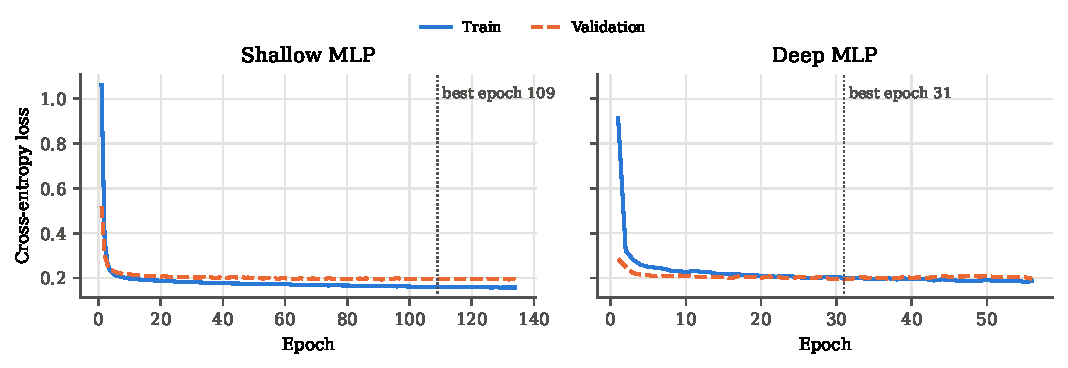
\includegraphics[width=\textwidth]{mlp_loss_curves.pdf}
\caption{Training and validation loss for both MLP variants. The dotted line marks the epoch whose weights were kept.}
\label{fig:loss}
\end{figure*}

\subsection{Data Split}
I first removed 68 exact duplicate rows, leaving 13,543 grains, so no bean could appear in both training and test. I then made a stratified 70/15/15 split with seed 42: 9,479 training, 2,032 validation and 2,032 test grains. Stratifying matters because the classes are unbalanced: Bombay is under 4\% of the data and Dermason about 26\%.

Area is in the tens of thousands of pixels while Roundness is between 0 and 1, so I standardized the features with a \texttt{StandardScaler} fit on the training set only. All model selection used the validation set. The test set was used once, at the end.

\subsection{Traditional Classifier}
I tuned all five classifiers from the assignment with scikit-learn \cite{pedregosa2011sklearn}: logistic regression, $k$-nearest neighbours, a decision tree, a random forest and an SVM. Each had a small grid of 5 to 28 configurations, trained on the training set and scored by validation macro-F1. The SVM grid included the kernel (linear, RBF and polynomial).

The SVM scored highest (Table~\ref{tab:screening}) with C=10, gamma=0.1, kernel=rbf. I did not refit it on training plus validation data, so both final models were trained on the same 9,479 grains.

\begin{table}[!t]
\centering
\caption{Validation results for the best configuration of each traditional classifier. The chosen model is in bold.}
\label{tab:screening}
\begin{tabular}{lccr}
\toprule
Classifier & Val. acc. & Val. macro-F1 & Tuning (s) \\
\midrule
\textbf{SVM} & 0.9272 & 0.9385 & 22.3 \\
k-NN & 0.9218 & 0.9329 & 0.7 \\
Logistic regression & 0.9222 & 0.9315 & 1.8 \\
Random forest & 0.9188 & 0.9304 & 19.7 \\
Decision tree & 0.9144 & 0.9237 & 2.4 \\
\bottomrule
\end{tabular}
\end{table}

\subsection{Neural Network}
The network is the \texttt{SimpleMLP} from class with 16 inputs and 7 outputs. Each hidden layer is a linear layer and a ReLU, optionally followed by dropout. I compared two variants:
\begin{itemize}
\item \textbf{Shallow:} one hidden layer of 64 units (1,543 parameters).
\item \textbf{Deep:} hidden layers of 128, 64 and 32 units, each followed by dropout of 0.2 (12,743 parameters).
\end{itemize}
Both used cross-entropy loss, Adam \cite{kingma2015adam} with a learning rate of 0.001, batches of 64, and up to 300 epochs. Training stopped after 25 epochs without improvement in validation loss, and the best epoch's weights were kept.

\begin{table}[!t]
\centering
\caption{MLP variants on the validation set. The chosen variant is in bold.}
\label{tab:variants}
\resizebox{\columnwidth}{!}{\begin{tabular}{lcrcccr}
\toprule
Variant & Hidden & Params & Val. acc. & Val. F1 & Best ep. & Time (s) \\
\midrule
\textbf{shallow} & [64] & 1,543 & 0.9291 & 0.9413 & 109 & 21.0 \\
deep & [128,64,32], p=0.2 & 12,743 & 0.9296 & 0.9392 & 31 & 13.0 \\
\bottomrule
\end{tabular}}
\end{table}

The shallow network had the higher validation macro-F1 (0.9413 against 0.9392; Table~\ref{tab:variants}), though the deep one had slightly higher accuracy. In Fig.~\ref{fig:loss}, the shallow network's validation loss improved slowly until epoch 109, while the deep network reached its lowest validation loss at epoch 31. The deep network's training loss is above its validation loss for the first half of training, because dropout is only active during training. With the scores this close, I chose the shallow network, which has about 8 times fewer parameters.

\section{Results}

\begin{figure*}[!t]
\centering
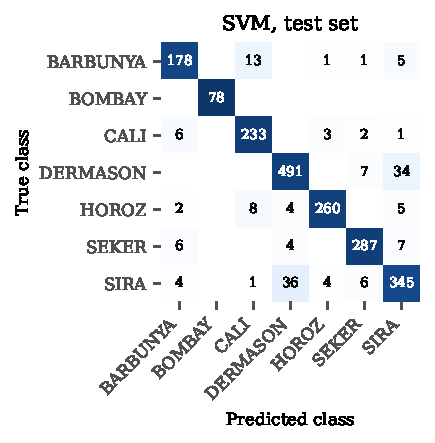
\includegraphics[width=0.4\textwidth]{confusion_classical.pdf}\hspace{0.06\textwidth}
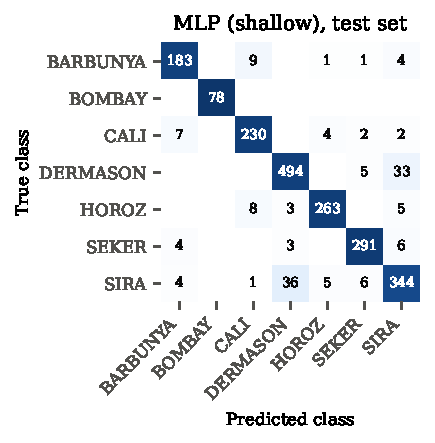
\includegraphics[width=0.4\textwidth]{confusion_mlp.pdf}
\caption{Test set confusion matrices for the SVM (left) and the MLP (right). Cell shading is row-normalized (per-class recall); numbers are raw counts.}
\label{fig:confusion}
\end{figure*}

On the 2,032 test grains (Table~\ref{tab:test}), the MLP (shallow) reached 92.67\% accuracy and 0.9374 macro-F1, and the SVM reached 92.13\% and 0.9318. That is 149 errors for the MLP and 160 for the SVM. The MLP's per-class F1 is equal or higher for every class, by less than 0.002 for Cali and Sira. Koklu and \"Ozkan \cite{koklu2020drybean} reported 93.13\% accuracy for an SVM on this dataset, but with a different evaluation setup, so the numbers are not directly comparable.

\begin{table}[!t]
\centering
\caption{Test set results for the two final models.}
\label{tab:test}
\begin{tabular}{lcc}
\toprule
Metric & SVM & MLP (shallow) \\
\midrule
Accuracy & 0.9213 & 0.9267 \\
Macro-F1 & 0.9318 & 0.9374 \\
\midrule
\multicolumn{3}{l}{\textit{Per-class F1}} \\
BARBUNYA & 0.9036 & 0.9242 \\
BOMBAY & 1.0000 & 1.0000 \\
CALI & 0.9320 & 0.9331 \\
DERMASON & 0.9203 & 0.9251 \\
HOROZ & 0.9506 & 0.9529 \\
SEKER & 0.9456 & 0.9557 \\
SIRA & 0.8701 & 0.8709 \\
\bottomrule
\end{tabular}
\end{table}

Both models classify Bombay perfectly (Fig.~\ref{fig:confusion}). Most other errors fall in two pairs. Sira and Dermason were confused 36 and 34 times by the SVM and 36 and 33 times by the MLP. Barbunya was predicted as Cali 13 times by the SVM and 9 times by the MLP.

\section{Discussion}
The MLP did better, but only by 149 errors against 160 out of 2,032, on one split. The validation gaps were similarly small, so another seed could reverse the order. I treat the two models as roughly equal.

\subsection{Features limit accuracy}
Apart from the decision tree, every traditional classifier scored between 0.9304 and 0.9385 validation macro-F1 (Table~\ref{tab:screening}), and both MLPs were only slightly higher. A linear SVM reached 0.9327 against 0.9385 for the RBF kernel, so the classes are close to linearly separable and a non-linear boundary helps only a little. Very different models reaching the same score points to a limit in the features rather than in any one model.

The confusion matrices support this. Both models make the same mistakes, mainly Sira with Dermason and Barbunya with Cali. These pairs seem to have similar sizes and outlines, so their 16 features overlap. Bombay is the opposite: it is much larger than the other varieties and its area barely overlaps theirs, so both models get it right.

\subsection{Model size and data}
With 9,479 training grains and 16 features, this is a small problem for a neural network. The shallow MLP has 1,543 parameters, about 6.1 training examples per parameter. The deep variant's 12,743 parameters gave no improvement. The SVM kept 1,720 support vectors (27,520 stored values), so the two final models are of similar size. With only 16 inputs, extra depth had little to add.

\subsection{Training time and tuning}
Training was fast for both. The final SVM fit took 0.37~s, and the 28-configuration SVM search took 22.3~s. Both MLP variants together took 34.0~s on a CPU. The SVM was much more sensitive to its settings: its worst configuration scored 0.3224 macro-F1. Both MLPs worked well with default Adam settings, and early stopping chose the number of epochs, so the MLP needed less tuning.

\subsection{Interpretability}
Neither model is easy to inspect directly. The SVM's decisions depend on 1,720 support vectors, and the MLP's on 1,543 weights. Logistic regression and a decision tree are easier to read, and both were within 0.015 validation macro-F1 of the SVM, which may be worth the small loss in accuracy.

To compare the two on the same terms, I used permutation importance on the validation set (Fig.~\ref{fig:importance}). Both models rely most on Roundness. The SVM then relies mostly on ShapeFactor4, while the MLP also uses Area, AspectRatio, ShapeFactor1 and ShapeFactor2. Area, ConvexArea, Perimeter and EquivDiameter are highly correlated (0.97 to 1.00), so shuffling one leaves the others available, and this method likely understates how much both models depend on size.

\begin{figure}[!t]
\centering
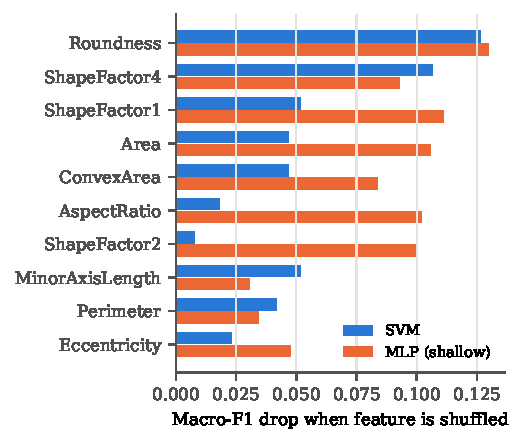
\includegraphics[width=0.9\columnwidth]{feature_importance.pdf}
\caption{Permutation importance on the validation set: the drop in macro-F1 when one feature is shuffled (top 10 features).}
\label{fig:importance}
\end{figure}

\section{Conclusion}
The best traditional classifier was an RBF SVM, and the best network was a shallow MLP with one hidden layer of 64 units. On the test set, the MLP reached 92.67\% accuracy and 0.9374 macro-F1, against 92.13\% and 0.9318 for the SVM. The gap is too small to call either model better.

The choice of model mattered less than the features. Apart from the decision tree, every model scored within about one point of macro-F1 of the others, and the SVM and MLP confused the same varieties. A model working from these 16 size and shape features cannot use information the features leave out.

With more time, I would try:
\begin{itemize}
\item A CNN on the original bean images, which could use texture and surface detail that the current features discard.
\item Repeated splits or cross-validation, to check whether the gap between the MLP and SVM is real.
\item A class-weighted loss for the MLP.
\end{itemize}


\bibliographystyle{IEEEtran}
\bibliography{refs}

\end{document}
